\chapter{\acl{mipwa}}
\label{chap:model_independent_pwa}

    \section{What I have developed}

    \section{Tests of model-independent partial-wave analysis}
    \ac{mipwa} allows for a description of waves whose resonance content is not yet well known or whose resonance shapes are not yet precisely understood.
    As an example, \citeauthor{PhysRevD.73.032004}~\cite{PhysRevD.73.032004} already employed \ac{mipwa} in the measurement of S-wave amplitudes for $\PDplus\to\PKminus\Ppiplus\Ppiplus$ decays at Fermilab.
    \citeauthor{Link200914}~\cite{Link200914} for the {\small FOCUS} collaboration also conducted a similar study on the same hadronic decay.


    As of writing, \pac{yap} does yet not allow for a proper handling of \ac{mipwa} fits.
    I implemented a \ac{mipwa} by adding a new dynamic shape that is indeed a characteristic function on a right-open range mass $M = [m_\textup{min}, m_\textup{max})$, which means:
    \begin{equation}
        B_M(m) = 
        \begin{cases}
            1 &\text{if }m\in M, \\
            0 &\text{otherwise}.
        \end{cases}
    \end{equation}
    The mass range of the Dalitz plot is then partitioned in $N_\text{bins}$ number of bins and $N_\text{bins}$ artificial decaying particles with characteristic functions as dynamic shapes are added to the \lstinline!DecayChannel!.
    Each of this particles adds a complex parameter to the fit so that, in total, $N_\text{bins}$ free real amplitude pairs $(\rho_i,\phi_i)$ need to be fitted.


    To test this approach I have fitted (what?) to a data set generated by a \pac{bat}'s \ac{mc} engine.
    In the figure~\ref{fig:mi_test_data} I simulated a $\PDplus\to\Ppiplus\Ppiminus\Ppiplus$ decay with only one resonance, namely $\Pfz\to\Ppiplus\Ppiminus$.
    The specific resonance I have chosen is not important here, I only chose it because it's spinless.
    In the plot, I have set its width to \SI{280}{\mega\electronvolt}, which is four times the particle's width value, to have enough events in all the bins and agevolate the fit.


    In the figure~\ref{fig:mi_test_fit_amp_8bins} I performed a fit by partitioning the mass range in eight equally-wide bins.
    The Breit-Wigner structure is reproduced.




    In the first fit attempt, I represented the complex fit parameters with their real and imaginary parts.
    With this choice, the pre-run did not converge as there is an ambiguity in the sign of the imaginary part of the parameters.
    In fatc, for each set of parameters $\Set{(\Re,\Im)_i}$ that maximizes the likelihood, also $\Set{(\Re,-\Im)_i}$ does.


    When representing the fit parameters in terms of magnitude and fase, the ambiguity remains.
    Moreover, \pac{bat} cannot properly handle the phase periodicity so the phase-space sampling becomes inefficient.
    To get rid of the sign ambiguity in the phase, I have chosen the fit parameters to be the magnitude of the bin free amplitudes and the phase difference between each bin's free amplidude and the previous bin's one.
    Namely the fit parameters are $P_i = (\rho_i, \uD\phi_i)$, where $\rho_i$ is the free-amplitude magnitude of the $i$-th bin, $\abs{A_i}$, and $\uD\phi_i = \phi_i - \phi_{i-1}$ is the difference between two adjacent bin's free-amplitude phases. 
    The phase ambiguity is removed by enforcing each fit parameter $\uD\phi_i$ to be non-negative.
    Note that by convention the first phase difference is set to zero:
    \begin{equation}\label{eq:delta_phi_zero_cond}
        \uD\phi_0 \coloneqq 0.
    \end{equation}

    During the fit I have noticed that the convergence takes longer for the phase-difference parameters than for the magnitude parameters to be reached.

    \subsection{Fit runtime}


    \begin{figure}
        \centering
        \begin{tikzpicture}
            \begin{semilogyaxis} [
                    xlabel = {Number of bins},
                    ylabel = {Runtime [\si{\hour}]}
                ]
                \addplot+ table {data/time_scale.dat};
            \end{semilogyaxis}
        \end{tikzpicture}
        \caption{Fit runtimes as a function of the number of bins in the allowed mass range.}
        \label{fig:time_scale}
    \end{figure}

    The figure~\ref{fig:time_scale} shows the time scaling of the fit with the number of bins.
    The rumtime increases exponentially when the number of bins grows.
    Note that each bin adds two real \acp{dof} to the fit so that
    \begin{equation}
        N_\text{DOF} = 2(N_\text{bins} - 1).
    \end{equation}
    One of the \acp{dof} is always fixed by the condition~\eqref{eq:delta_phi_zero_cond}.
    \begin{figure}
        \centering
        \begin{tikzpicture}
    \begin{axis}[
            error bars/y dir=both,
            error bars/y explicit,
            xlabel = {Bin index},
            ylabel = {Amplitude}
        ]
        \addplot+[ybar stacked] table [x index=0, y index=1, y error index=2] {data/output8bins/parameters.dat};
        %\addplot+[ybar stacked] table [x index=0, y index=1, y error index=2] {data/output8bins/parameters.dat};
    \end{axis}
\end{tikzpicture}

        \caption{Breit-Wigner fitted with eight equally-spaced bins using \pac{bat}.
                 The secont bin's free amplitude magnitude is fixed to \num{1}.}
        \label{fig:mi_test_fit_amp_8bins}
    \end{figure}
    I usually fix the other \ac{dof} by setting the magnitude of some free amplitude to \num{1}, \eg{}~in figure~\ref{fig:mi_test_fit_amp_8bins} I fixed the second bin's free amplitude.


\begin{figure}
    \centering
    %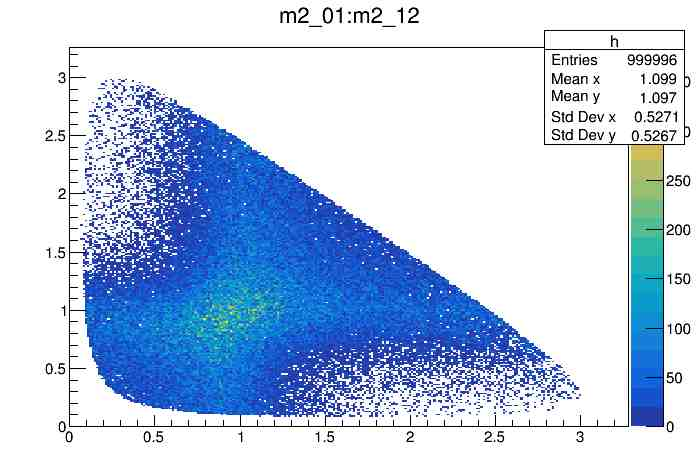
\includegraphics[width=.9\textwidth]{fig/toy_example.pdf}
    \caption{\ac{mc}-generated data set for testing the \ac{mipwa} approach in \pac{yap}.}
    \label{fig:mi_test_data}
\end{figure}

    \subsection{Pre-run exceptions}

    {\color{red} Why?
    To fit a model to some data, a pre-run must be done(?).
    }

    I noticed that \pac{bat} crashed in the pre-run phase if I tried to generate initial point when the mass-width of the bins was \SI{45.3}{\mega\electronvolt}.

    Generating initial points works with a bin width of \SI{60.5}{\mega\electronvolt} but fails with \SI{45.3}{\mega\electronvolt}.
    Can this maybe depend on the number of parameters?

    \begin{lstlisting}
terminate called after throwing an instance of 'std::runtime_error'
  what():  BCEngineMCMC::MCMCInitialize : Could not generate uniformly distributed initial point with valid probability in 10000000 tries.
  zsh: abort (core dumped)  ./runBatFit
    \end{lstlisting}


    \begin{figure}
        \centering

        \subfloat[][\label{fig:f0_phase_fit}]{\begin{tikzpicture}
    \begin{axis}[phase_plot]

    \addplot+ [guess] table [x index={0}, y index={5}]
              {data/f0_f0_1500_sigma_rho0/s_par_guess.txt};
    \addplot+ [fit] table [x index={0}, y index={5}, y error index={6}]
              {data/f0_f0_1500_sigma_rho0/s_par_fit.txt};
    \end{axis}
\end{tikzpicture}
}

        \subfloat[][]{\begin{tikzpicture}
    \begin{axis}[amplitude_plot]

        \addplot+ [guess] table [x index={0}, y index={1}]
                  {data/f0_f0_1500_sigma_rho0/s_par_guess.txt};
        \addplot+ [fit, error bars/.cd, y dir=both, y explicit]
            table [x index={0}, y index={1}, y error index={2}]
                  {data/f0_f0_1500_sigma_rho0/s_par_fit.txt};
    \end{axis}
\end{tikzpicture}
}

        \caption{Freed-wave fit of the S wave of a $\PDplus \to \Ppiplus\Ppiminus\Ppiplus$ decay through the \Pfnez{} resonance.} 
        \label{fig:f0_fit}
    \end{figure}

    \begin{figure}
        \centering

        \subfloat[][Here the effect of the non-negative phase motion is visible. Due to a misidentification of the second phase value, the phases up to \SI{1}{\giga\electronvolt} are systematically shifted up.]{\begin{tikzpicture}
    \begin{axis}[phase_plot]

    \addplot+ [guess] table [x index={0}, y index={5}]
              {data/f0_f0_1500_sigma_rho0_f2/d_par_guess.txt};
    \addplot+ [fit] table [x index={0}, y index={5}, y error index={6}]
              {data/f0_f0_1500_sigma_rho0_f2/d_par_fit.txt};
    \end{axis}
\end{tikzpicture}
}

        \subfloat[][In the end of the phase space, the angular dependency becomes small. This introduces an ambiguity in the phase also.]{\begin{tikzpicture}
    \begin{axis}[amplitude_plot]

        \addplot+ [guess] table [x index={0}, y index={1}] {data/f0_f2/d_par_guess.txt};
        \addplot+ [fit, error bars/.cd, y dir=both, y explicit]
            table [x index={0}, y index={1}, y error index={2}]
                  {data/f0_f2/d_par_fit.txt};
    \end{axis}
\end{tikzpicture}
}

        \caption{Freed-wave fit of the D wave of a $\PDplus \to \Ppiplus\Ppiminus\Ppiplus$ decay through the \Pfii{} resonance.}
    \end{figure}

    \begin{figure}
        \centering
        \subfloat[][Source data: decay in the S and D wave through the \Pfnez{} and \Pfii{} resonances.]{\begin{tikzpicture}
    \begin{axis} [dalitz_plot]

        \addplot3 [dalitz]
          gnuplot [raw gnuplot] { splot "data/f2/f2_mcmc.txt" using 1:2:3 };
    \end{axis}
\end{tikzpicture}
}

        \subfloat[][Result of the model-independent fit to the plot shown above.]{\begin{tikzpicture}
    \begin{axis} [dalitz_plot]
        \addplot3 [dalitz]
          gnuplot [raw gnuplot]
                  { splot "data/f0_f0_1500_sigma_rho0/f0_f0_1500_sigma_rho0_fit_result_mcmc.txt" using 1:2:3 };
    \end{axis}
\end{tikzpicture}
}
        \caption{\ac{mc}-generated Dalitz plots of a $\PDplus \to \Ppiplus\Ppiminus\Ppiplus$ decay.}
    \end{figure}


    \begin{figure}
        \centering

        \subfloat[][Unlike the phase fit~\ref{fig:f0_phase_fit}, to perform this fit, I had to allow the negative values for the phase motion.]{\begin{tikzpicture}
    \begin{axis}[phase_plot]
        \addplot+ [guess] table [x index={0}, y index={5}] {data/f2/par_guess.txt};
        \addplot+ [fit] table [x index={0}, y index={5}, y error index={6}]
                  {data/f2/par_fit.txt};

    \end{axis}
\end{tikzpicture}
}

        \subfloat[][Sum of two Breit-Wigner mass shapes with zero relative phase.]{\begin{tikzpicture}
    \begin{axis}[amplitude_plot]
        \addplot+ [guess] table [x index={0}, y index={1}] {data/f0/par_guess.txt};
        \addplot+ [fit] table [x index={0}, y index={1}, y error index={2}]
                  {data/f0/par_fit.txt};
    \end{axis}
\end{tikzpicture}

}

        \caption{Freed-wave fit of the S wave of a $\PDplus \to \Ppiplus\Ppiminus\Ppiplus$ decay through the \Pfnez{} and \Pfofzz{} resonances.}
    \end{figure}

    \begin{figure}
        \centering
        \subfloat[][Source data: S-wave decay through the \Pfnez{} and \Pfofzz{} resonances.]{\begin{tikzpicture}
    \begin{axis} [dalitz_plot]

        \addplot3 [dalitz]
          gnuplot [raw gnuplot] { splot "data/f2/f2_mcmc.txt" using 1:2:3 };
    \end{axis}
\end{tikzpicture}
}

        \subfloat[][Result of the model-independent fit to the plot shown above.]{\begin{tikzpicture}
    \begin{axis} [dalitz_plot]
        \addplot3 [dalitz]
          gnuplot [raw gnuplot]
                  { splot "data/f0_f0_1500_sigma_rho0/f0_f0_1500_sigma_rho0_fit_result_mcmc.txt" using 1:2:3 };
    \end{axis}
\end{tikzpicture}
}

        \caption{\ac{mc}-generated Dalitz plots of a $\PDplus \to \Ppiplus\Ppiminus\Ppiplus$ decay.}
    \end{figure}

    \begin{figure}
        \centering

        \subfloat[][]{\begin{tikzpicture}
    \begin{axis}[phase_plot]
        \addplot+ [guess] table [x index={0}, y index={5}] {data/f2/par_guess.txt};
        \addplot+ [fit] table [x index={0}, y index={5}, y error index={6}]
                  {data/f2/par_fit.txt};

    \end{axis}
\end{tikzpicture}
}

        \subfloat[][]{\begin{tikzpicture}
    \begin{axis}[amplitude_plot]
        \addplot+ [guess] table [x index={0}, y index={1}] {data/f0/par_guess.txt};
        \addplot+ [fit] table [x index={0}, y index={1}, y error index={2}]
                  {data/f0/par_fit.txt};
    \end{axis}
\end{tikzpicture}

}


        \caption{Freed-wave fit of the P wave of a $\PDplus \to \Ppiplus\Ppiminus\Ppiplus$ decay through the \Prhozero{} resonance.}
    \end{figure}

    \begin{figure}
        \centering
        \subfloat[\acs{mc}-generated Dalitz plot of a P-wave decay through the \Prhozero{} resonance.]%
                 [Source data: P-wave decay through the \Prhozero{} resonance.]%
                 {\begin{tikzpicture}
    \begin{axis} [dalitz_plot]

        \addplot3 [dalitz]
          gnuplot [raw gnuplot] { splot "data/f2/f2_mcmc.txt" using 1:2:3 };
    \end{axis}
\end{tikzpicture}
}

        \subfloat[\acs{mc}-generated Dalitz plot of a P-wave decay through the \Prhozero{} resonance.]%
                 [Result of the model-independent fit to the plot shown above.]%
                 {\begin{tikzpicture}
    \begin{axis} [dalitz_plot]
        \addplot3 [dalitz]
          gnuplot [raw gnuplot]
                  { splot "data/f0_f0_1500_sigma_rho0/f0_f0_1500_sigma_rho0_fit_result_mcmc.txt" using 1:2:3 };
    \end{axis}
\end{tikzpicture}
}

        \caption{\ac{mc}-generated Dalitz plots of a P-wave $\PDplus \to \Ppiplus\Ppiminus\Ppiplus$ decay through the \Prhozero{} resonance.}

    \end{figure}

    \begin{figure}
        \centering

        \subfloat[][]{\begin{tikzpicture}
    \begin{axis}[phase_plot]
        \addplot+ [guess] table [x index={0}, y index={5}] {data/f2/par_guess.txt};
        \addplot+ [fit] table [x index={0}, y index={5}, y error index={6}]
                  {data/f2/par_fit.txt};

    \end{axis}
\end{tikzpicture}
}

        \subfloat[][\label{fig:f2_amplitude}]{\begin{tikzpicture}
    \begin{axis}[amplitude_plot]
        \addplot+ [guess] table [x index={0}, y index={1}] {data/f0/par_guess.txt};
        \addplot+ [fit] table [x index={0}, y index={1}, y error index={2}]
                  {data/f0/par_fit.txt};
    \end{axis}
\end{tikzpicture}

}


        \caption{Freed-wave fit of the D wave of a $\PDplus \to \Ppiplus\Ppiminus\Ppiplus$ decay through the \Pfii{} resonance.}
    \end{figure}

    \begin{figure}
        \centering
        \subfloat[]%
                 [Source data: D-wave decay through the \Pfii{} resonance.\label{fig:f2_dalitz_source}]%
                 {\begin{tikzpicture}
    \begin{axis} [dalitz_plot]

        \addplot3 [dalitz]
          gnuplot [raw gnuplot] { splot "data/f2/f2_mcmc.txt" using 1:2:3 };
    \end{axis}
\end{tikzpicture}
}

        \subfloat[]%
                 [Result of the model-independent fit to the plot shown above.]%
                 {\begin{tikzpicture}
    \begin{axis} [dalitz_plot]
        \addplot3 [dalitz]
          gnuplot [raw gnuplot]
                  { splot "data/f0_f0_1500_sigma_rho0/f0_f0_1500_sigma_rho0_fit_result_mcmc.txt" using 1:2:3 };
    \end{axis}
\end{tikzpicture}
}

        \caption{\ac{mc}-generated Dalitz plots of a $\PDplus \to \Ppiplus\Ppiminus\Ppiplus$ decay.}

    \end{figure}

    The determination of the phase motion is much easier for the S wave than it is for other waves, due to their non-trivial angular dependency.
    \begin{figure}
        \centering
        \begin{tikzpicture}
    \begin{axis}[
            phase_plot,
            ylabel={Dynamic-shape phase motion $[\si{deg}]$}
        ]
        \addplot+ [guess] table [x index={0}, y index={3}] {data/f2/par_guess.txt};
        \addplot+ [fit] table [x index={0}, y index={3}, y error index={4}]
                  {data/f2/par_fit.txt};

    \end{axis}
\end{tikzpicture}

        \caption{Phase motion of the \Pfii{} fit. The phase motion of the first bin is fized to zero.}
        \label{fig:fit_f2_phase_motion}
    \end{figure}
    The figure~\ref{fig:fit_f2_phase_motion} shows a comparison between the fitted phase phase motion for the \Pfii{} resonance in the Dalitz plot~\ref{fig:f2_dalitz_source}. 
    The last two phase motions are not precisely determined due to the effect of the wave angular dependency, which tends to suppress the decay amplitude at the end of the phase space. 
    The decay-amplitude dumping makes the fit ambiguous in that area of the Dalitz plot.
    This effect can also be seen in the amplitude plot~\ref{fig:f2_amplitude}.


    The same holds for the P-wave \Prhozero{} fit.


    \subsection{Likelihood function}

    The model-independent fit to the \ac{mc}-generated data set, $D = \Set{d_1, d_2,\dots, d_m}$, is performed through the maximum-likelihood method.
    In this section I am going to justify the expression of the log-likelihood used in the fittin routine.

    If $p \coloneqq (p_1, p_2,\dots, p_n)$ is the fit-parameter vector, the Bayes' theorem reads
    \begin{equation}
        P(p\given D) = \frac{P(D\given p)\, P(p)}{P(D)}.
    \end{equation}
    First, let's note that the parameters are assumed to be independent among each other, so that
    \begin{equation}
        P(p) = \prod_{i = 1}^n P_i(p_i),
    \end{equation}
    being $P_i$ the probability density function of the $i$-th parameter.
    As there is no information about the fit parameters, I choose the following flat distributions for the priors:
    \begin{equation}\label{eq:flat_priors}
        P_i(p_i) =
        \begin{cases}
            1/(b_i - a_i) & \text{if } a_i \le p_i \le b_i, \\
            0             & \text{otherwise},
        \end{cases}
    \end{equation}
    where $[a_i, b_i]$ is the domain of the $i$-th parameter.
    This choice implies that the prior $P(p)$ is a constant function in the hypercube where all its arguments are defined.

    The likelihood function is defined as the conditional probability of observing the data set $D$ given $p$, that is
    \begin{equation}
        L(p) \coloneqq P(D\given p).
    \end{equation}
    Since the priors and $P(D)$ are constant functions, the likelihood is directly proportional to the posterior probability:
    \begin{equation}
        P(p\given D) = \alpha L(p),\quad \text{where } \alpha \coloneqq \frac{P(p)}{P(D)}.
    \end{equation}
    The logarithm of the likelihood reads
    \begin{equation}
        \log L(p) = \log P(p\given D) - \log \alpha.
    \end{equation}


    The posterior probability is proportional to the square magnitude of the decay amplitude, which is the model \emph{intensity}\index{intensity}.
    This is a function of the decay phase-space point $\mu$ defined as follows:
    \begin{equation}
        I_p(\mu) \coloneqq \abs{\A_p(\mu)}^2.
    \end{equation}
    With this definition, the posterior probability of the fit parameters given an observed point in the phase space, $d$, is
    \begin{equation}
        P(p\given d) = \frac{I_p(d)}{\displaystyle\int I_p(\mu)\ud\mu},
    \end{equation}
    where the normalizing integral is over the whole decay phase-space.
    Assuming the point in the observed data set have no correlation, the posterior for the fit parameters given the whole set $D$ is
    \begin{equation}
        P(p\given D) = \prod_{d\in D} P(p\given d) = \frac{\displaystyle\prod_{d\in D}I_p(d)}{\displaystyle\left(\int I_p(\mu)\ud\mu\right)^m}.
    \end{equation}
    The log-likelihood then reads
    \begin{equation}
        \log L(p) = \sum_{d\in D}\log I_p(d) - m\log\int I_p(\mu) \ud \mu - \log \alpha.
    \end{equation}
    Retaining only the $p$-dependent terms in the equation above, the expression of the log-likelihood that needs to be maximized is
    \begin{equation}\label{eq:log_lik_unstable}
        \log \tilde L(p) = \sum_{d\in D}\log I_p(d) - m\log \int I_p(\mu)\ud\mu.
    \end{equation}


    It is worth pointing out that, in the fit routine, the expression used for the log-likelihood is the following:
    \begin{equation}\label{eq:log_lik_stable}
        \log \tilde L(p) = \sum_{d\in D}\left(\log I_p(d) - \log \int I_p(\mu)\ud\mu\right)\!.
    \end{equation}
    In fact, while being mathematically equivalent, the~\eqref{eq:log_lik_stable} is numerically more stable than the~\eqref{eq:log_lik_unstable}.


